\section{سوال دوم}
در این بخش به هدایت  پهپاد به روش تناسی خالص و غیرخطی پرداخته شده است. بر اساس صورت سوال، روش هدایت در حالت‌های مختلف تغیر می‌کند.
در شبیه‌سازی از \lr{State Flow}
جهت تعین روش هدایت استفاده شده است. 
\subsection{بخش الف}
بر اساس شرایط اشاره در صورت سوال شبیه‌سازی انجام شده و نتایج آن در شکل \ref{fig:q2_1} آمده است. همانطور که مشاهده می‌شود در این حالت پهپاد به سمت هدف حرکت می‌کند و در نهایت به آن می‌رسد.
\begin{figure}[H]
    \label{fig:q2_1}
	\centering
	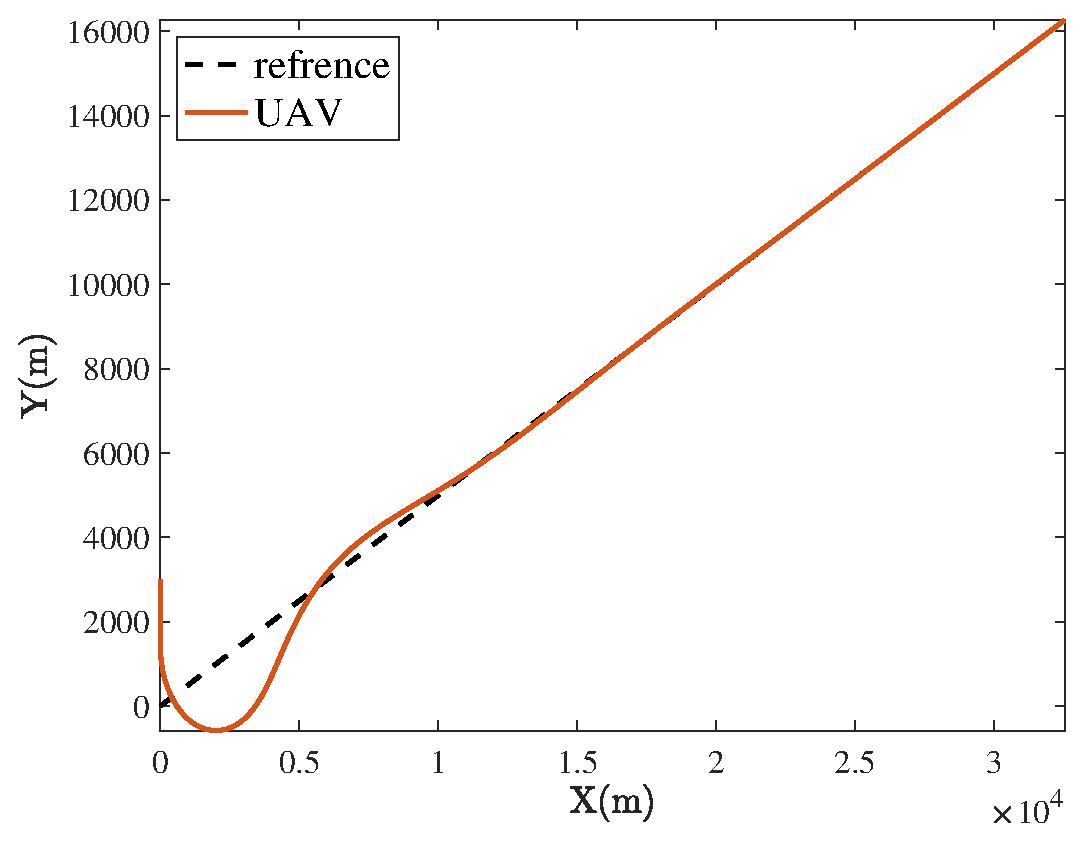
\includegraphics[width=.75\linewidth]{../Figure/Q2/a/xy}
	\caption{موقعیت پهپاد در صفحه X-Y  }
\end{figure}

\begin{figure}[H]
    \label{fig:q2_1}
	\centering
	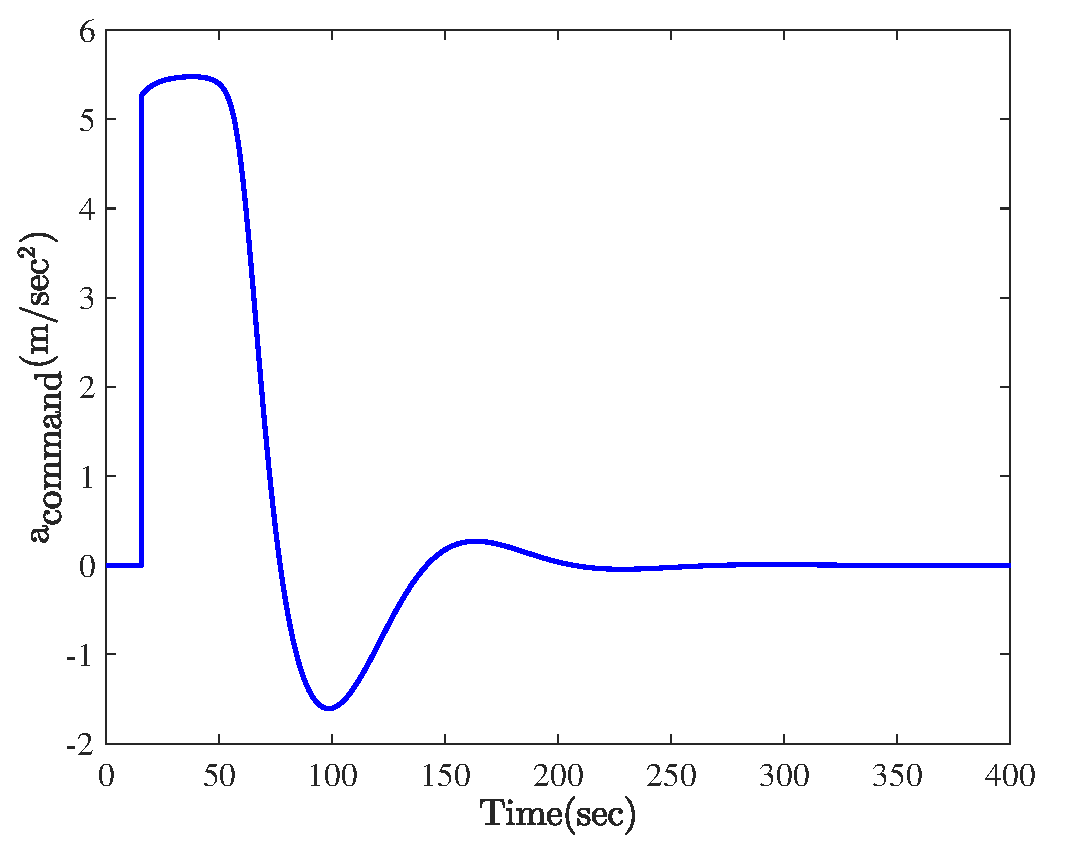
\includegraphics[width=.75\linewidth]{../Figure/Q2/a/acc}
	\caption{فرمان هدایت به‌صورت تابعی از زمان}
\end{figure}


